% !TEX TS-program = pdflatex
% !TEX encoding = UTF-8 Unicode

% This is a simple template for a LaTeX document using the "article" class.
% See "book", "report", "letter" for other types of document.

\documentclass[11pt]{article} % use larger type; default would be 10pt

\usepackage[utf8]{inputenc} % set input encoding (not needed with XeLaTeX)

%%% Examples of Article customizations
% These packages are optional, depending whether you want the features they provide.
% See the LaTeX Companion or other references for full information.

%%% PAGE DIMENSIONS
\usepackage{geometry} % to change the page dimensions
\geometry{a4paper} % or letterpaper (US) or a5paper or....
\geometry{margin=1in} % for example, change the margins to 2 inches all round
% \geometry{landscape} % set up the page for landscape
%   read geometry.pdf for detailed page layout information

\usepackage{graphicx} % support the \includegraphics command and options

% \usepackage[parfill]{parskip} % Activate to begin paragraphs with an empty line rather than an indent

%%% PACKAGES
\usepackage{booktabs} % for much better looking tables
\usepackage{array} % for better arrays (eg matrices) in maths
\usepackage{paralist} % very flexible & customisable itemizes (eg. enumerate/itemize, etc.)
\usepackage{verbatim} % adds environment for commenting out blocks of text & for better verbatim
\usepackage{subfig} % make it possible to include more than one captioned figure/table in a single float
\usepackage{amssymb} % more 'unusual' symbols not included in standard LaTeX package
\usepackage{enumitem}
\usepackage{amsmath}
\usepackage{xspace}
\usepackage{gensymb}
\usepackage{calligra} 
\DeclareMathAlphabet{\mathcalligra}{T1}{calligra}{m}{n} 
\DeclareFontShape{T1}{calligra}{m}{n}{<->s*[2.2]callig15}{} 

% These packages are all incorporated in the memoir class to one degree or another...

%%% HEADERS & FOOTERS
\usepackage{fancyhdr} % This should be set AFTER setting up the page geometry
\pagestyle{fancy} % options: empty , plain , fancy
\renewcommand{\headrulewidth}{0pt} % customise the layout...
\lhead{}\chead{}\rhead{}
\lfoot{}\cfoot{\thepage}\rfoot{}

%%% SECTION TITLE APPEARANCE
\usepackage{sectsty}
\allsectionsfont{\sffamily\mdseries\upshape} % (See the fntguide.pdf for font help)
% (This matches ConTeXt defaults)

%%% ToC (table of contents) APPEARANCE
\usepackage[nottoc,notlof,notlot]{tocbibind} % Put the bibliography in the ToC
\usepackage[titles,subfigure]{tocloft} % Alter the style of the Table of Contents
\renewcommand{\cftsecfont}{\rmfamily\mdseries\upshape}
\renewcommand{\cftsecpagefont}{\rmfamily\mdseries\upshape} % No bold!

%%%Command Macros
\newcommand{\vf}{\ensuremath{V_{F}}\xspace}
\newcommand{\sr}{\ensuremath{\mathcalligra{r}} \xspace}

%%% END Article customizations

\graphicspath{ {./images/} }

\title{The Mimas Leading Edge Anomaly: Thermal conductivity and grain cementation radius estimation}
\author{M.J. Schaible, R.Johnson, L. Zhigilei}
%\date{} % Activate to display a given date or no date (if empty),
         % otherwise the current date is printed 

\begin{document}
\maketitle

\section{Review of measured Parameters}
\label{sec:measured}

\subsection{Thermal Inertia (I) - Howett et al. (2011)}
\label{sec:inertia}

	\begin{equation}
	I = \sqrt{kc\rho} \: [\frac{J}{m^{2} K^{1} s^{1/2}}]
	\end{equation}

	\hspace{1cm}
	Where
	\begin{itemize}[leftmargin=3cm]
	\item k = thermal conductivity $[\frac{J}{m \cdot s \cdot K}]$
	\item c = specific heat $[\frac{J}{g \cdot K}]$
	\item $\rho$ = density $[\frac{g}{m^{3}}]$
	\end{itemize}

	The thermal inertial measured by Cassini CIRS was reported by Howett et al. (2011)
	\begin{itemize}
		\item Within anomaly: \fbox{$66 \pm 23  [\frac{J}{m^{2} K^{1} s^{1/2}}]$}
		\item Outside anomaly: \fbox{$< 16  [\frac{J}{m^{2} K^{1} s^{1/2}}]$}
	\end{itemize}
		
	\emph{Depth of penetration for CIRS wavelength light?}
	
\subsection{Temperature ranges - Howett et al. (2011)}
\label{sec:temperature}

	Estimated Mimas daytime temperatures: 40-95 K
	
\subsection{Particle Size - Hendrix et al (2012)}
\label{sec:size}

	Average particle diameter[$\mu$m]
	\begin{itemize}
	\item Leading hemisphere: 20-80 $\mu$m
	\item Trailing hemisphere: 10-50 $\mu$m
	\item Herschel crater: 50-100 $\mu$m
	\end{itemize}

\subsection{Porosity}
\label{sec:porosity}

	$\rho_{\phi} = \rho_{0}*(1-\phi)$

	\begin{itemize}
	\item For Enceladus - Verbischeret al (2005): $~50-70\%$
	\item For Tethy's - Caravano et al. (2007): $>90\%$ 
	\item Model parameter (ansatz) Leliwa-Kopystynski (2000): $~50\%$
	\end{itemize}

\section{Tabulated Literature Parameters}
\label{sec:tabulated}
	
\subsection{Thermal Conductivity}
\label{sec:tconductivity}
	
	Low temperature thermal conductivity
	
	\begin{itemize}
	\item Water Ice
		\begin{itemize}
		\item Ellsworty and Schubert (1983): $k_{ice} = \frac{488.12}{T} +0.4685 \: [\frac{J}{m s K}]$
		\item Haruyama et al (1993) via. Sirono and Yamamoto (1997):
			\begin{itemize}
			\item Amorphous: $k_{H_{2}O, a} = k_{ao} \times T$ where $k_{ao} = 7.1x10^{-3} \: [\frac{erg}{cm s K}]$
			\item Crystalline: $k_{H_{2}O, c} = k_{co}/T$ where $k_{co} = 5.67x10^{7} \: [\frac{erg}{cm s K}]$
			\end{itemize}
		\item Kossacki et al. (1994): $k = \frac{567}{T} \: [\frac{J}{m s K}]$
		\item Klinger (1975): $k_{100 K} = 0.04  \: \frac{J}{m s K}$ (amorphous)
		\end{itemize}
%	\item Silicates
%		\begin{itemize}
%		\item Basalt
%			\begin{itemize}
%			\item Clauser (1995) - Bulk: k $\approx 1.5 - 3.5 [ \frac{J}{m \cdot s \cdot K}]$
%			\item Fountain and West (1970) - Crushed (37-62 $\mu m, \rho = 0.9 g/cm^{3}$, T=150K): k $\approx 7\times10^{-4} [\frac{J}{m \cdot s \cdot K}]$
%			\end{itemize}
%		\item Quartz
%			\begin{itemize}
%			\item engineeringtoolbox.com - Bulk: k $\approx 3.0 [\frac{J}{m \cdot s \cdot K}]$
%			\item Smoluchowski (1910) - Crushed (94$\mu$m): k $\approx 3.0 [\frac{J}{m \cdot s \cdot K}]$
%			\end{itemize}
%		\item Pumice
%			\begin{itemize}
%			\item  Hemmings et al. (2009) - Bulk: k $\approx 0.4269 [\frac{J}{m \cdot s \cdot K}]$
%			\item Wechsler and Glaser (1965) - Crushed (44-104 $\mu$m): 
%			\end{itemize}
%		\end{itemize}
	\end{itemize}

\subsection{Specific  and Latent Heat}
\label{sec:sheat}

	Low temperature specific heat:
	
	\begin{itemize}
	\item Ramirez et al. (2012): $c_{100 K} ~ 0.83 [\frac{J}{g K}]$
	\item NBS Monograph 21 (): $c_{100 K} = 0.82 [\frac{J}{g K}]$
	\item Gutierrez et al. (2001): $c_{H_{2}O} = (0.9 + 0.00749 * T) [\frac{J}{g K}]$
	\end{itemize}
	
	Latent heat of sublimation:
	
	\begin{itemize}
	\item Gutierrez et al. (2001): $L = 48600 [\frac{J}{mol}]$
	\end{itemize}
	
\section{Comparison/Summary of thermal conductivity models}

	Here, several thermal conductivity models are discussed and it is seen that there are qualitative similarities shared by all; namely, that the models depend on the thermal conductivity of bulk ice, $k_{ice}$, the porosity, $\phi$, and on geometric factors that depend on the packing of grains. In each of the models, all contributions to thermal conductivity  other than conduction through grains (i.e. radiative, convective, latent heat) are taken to be zero. Conductivity through grains is limited by the contact area between adjacent grains. The models are discussed in more detail in the following and are presented here without modification from their orignal sources for ease of comparisson.
	
	\begin{itemize}
	\item Wood (2011, 2013)
		\begin{equation}
		\begin{split}
		k_{eff}  &= f_{sc} k_{ice} \frac{\chi + 1 - \phi}{\chi + 1 + \frac{\phi}{2}} \\
		&\text{Taking $\phi = 0.5$ and assuming $\chi << \phi$} \\
		\Rightarrow k_{eff} &\approx \frac{2}{5} f_{sc} k_{ice}
		\end{split}
		\end{equation}
	This equation requires that the $f_{sc}$ factor be fit to experimental data. The factor is a measure of the efficiency of contact between adjacent grains and is equivalent to geometrical+contact area. For uncemented soils, the factor is given in terms of the size and number of contacts, where contact size is determined by Hertzian analysis and cohesive surface forces (JKR theory) as in the following models. Wood is (apparently) developing an additional model that takes into account the cementation between grains. 
		
%	\item  Piqueuz and Christensen (2009b) \\
%		P and Q did not give explicit equations to calculate the thermal conductivity, but provided several larger plots that traced how the thermal conductivity varied with \% cementation, grain size, gas pressure etc. However, their focus was on ~atm pressure environments, and the model failed for very small grain contact areas (low thermal conductivities), and thus is was determined this model was unfit to explain the regolith at Mimas.

	\item Steiner and K\"{o}mle (1991)
		\begin{equation}
		\begin{split}
		 k_{eff} &= \sqrt{1-\phi}\cdot H \cdot k_{ice}(T) \\
		&\text{Taking $\phi = 0.5$} \\
		 k_{eff} &\approx 0.71 H k_{ice}
		\end{split}
		\end{equation}
	The Steiner and K\"omle model uses only the $\sqrt{1-\phi}$ factor to account the the structure of the material. The Hertz factor H is assumed to be similar to the other models. 

	\item Gundlach and Blum (2010)
		\begin{equation}
		\begin{split}
		k_{eff} = k_{ice} H \frac{1}{0.531 S(\vf)} \frac{N_{A}}{N_{L}} \\
		\text{where} H = [\frac{9}{4} \frac{1-\mu^{2}}{E} \pi \gamma r^{2} ]^{1/3}
		\end{split}
		\end{equation}
	The Gundlach and Blum model was developed using a mathematical analysis by Chan and Tien (1973) for regularly packed spheres whose contact area is described by Hertzian analysis and where the cohesive forces between spheres are described by JKR theory. The factors S$_{vf}$, N$_{A}$, and N$_{L}$ depend on the specific packing arrangement. Values are given for simple cubic, body centered cubic, and face centered cubic. Note that the porosity of a simple cubic lattice is 47.7\%, close to the 50\% porosity estimated for Mimas. 
	
	\item Sirono and Yamamoto (1997)
		\begin{equation}
		\begin{split}
		k_{eff} &= k_{ice} ( \frac{p - p_{c}}{1-p_{c}} )\frac{\pi \sr^{2}}{g r^{2}} \\
			 &= k_{ice} ( \frac{p - p_{c}}{1-p_{c}} )\frac{\pi}{g r^{2}}[ \frac{9 \pi \gamma r^{2} (1-\mu^{2})}{8 E} ]^{2/3}
		\end{split}
		\end{equation}
		Where \sr is the grain contact radius as defined by Hertzian analysis and 'p' is \underline{not} the volume filling factor, but related to it and dependent on the packing. 'p' is the probability that a lattice site is occupied with a regolith grain. 
	\end{itemize}

\newpage
\section{Introduction}
\label{sec:intro}

	Analysis of returned Cassini data revealed an anomalous region present on the leading edge of the icy moons of Mimas and Tethy's in the Saturnian system. The feature was seen first as a lens shaped darkening compared to the surrounding regions [Shenketal2011], seen most clearly by taking the ratio of IR/UV light, where the discoloration was centered a 0$\degree$ lat and 0$\degree$ long on the leading edge and extended $\sim \pm30\degree$ to the north and south while spreading over $\>180 \degree$ longitude. The smaller IR/UV ratio was explained as  increased scattering at UV wavelengths due to a higher concentration of defects in the icy regolith grains due to preferential bombardment of $\>$1 MeV electrons in this region.

	Later, using the CIRS instrument which measured light in the thermal IR regime, the emission from the surface was determined during the day and night cycle and it was seen that the temperature variation within a lens shaped region, closely matching the spatial extent of the IR/UV discoloration, was greater than the surrounding [Howettetal2011], indicating a greater thermal conductivity of the material. Both the discoloration and the anomalous thermal inertial have been tentatively explained by surface modifications that resulted from high energy (>1MeV) electrons traveling with the net guiding center of motion opposite the rotation direction of the moons and thereby depositing energy preferentially on the leading edge of those bodies [Paranicasetal2012]. (more?) The surfaces of the moons are composed almost entirely of crystalline water ice, while essentially free of organic species [Filacchioneetal2010], and the energy deposition due to these electrons was hypothesized to be responsible for an increased sintering volume between the ice grains.

	A good deal of thermal modeling has been done to understand the structure of comets and the thermal inertia of other bodies such as the Moon and Mars. However, unlike comets, the Saturn moons are not covered by a dark organic layer which eliminates thermal IR emission from the surface, and, in addition to being composed of water ice as opposed to a rocky regolith, the moons lack an atmosphere and thus the dominant thermal path is from grain contacts while the thermal conductivity due to gas convection is negligible. The purpose of this note is to quantitatively estimate the expected relative contact area or grain sintering radius based on the measured parameters of thermal inertia and grain size. The estimate assumes that both the ice grains and the cementation volume is entirely crystalline, although amorphous ice could be present. The structure of the ice will be discussed in more detail later in this note. 

\subsection{Skin Depth ($\delta$) - Howett et al. (2011)}

	Using the measured emission differences, the thermal inertia $I=\sqrt(kc\rho)$ was $16 \: J m^{-2} s^{-1/2} K^{-1}$ ouside the anomalous region and $66 \pm 23 \: J m^{-2} s^{-1/2} K^{-1}$ within.  Using these values Howett et al. gave a skin depth value of 
	
	\begin{equation}
	\begin{split}
	\delta_{out} &= \frac{I_{out}}{\rho_{regolith} c \sqrt{\omega}}  \\
		&= \frac{I_{out}}{(1-\phi)\rho_ {ice} c \sqrt{\omega}} \\
		&= \frac{16  [ \frac{J}{m^{2} s^{1/2} K} ]}{(1-0.5)0.934 [\frac{g}{cm^{3}}] 0.8 [\frac{J}{g \cdot K}] \sqrt{7.7\time10^{-5} [\frac{rad}{s}]}} \\
	\Rightarrow \delta_{out}&= 0.49\: [cm]
	\end{split}
	\end{equation}

	Where $c$ is specific heat, $\rho_{ice}$ is the density of bulk ice, $\phi$ is the porosity, taken here as 50\%, and $\omega$ the angular velocity of rotation. Inside the thermal anomaly the skin depth was given as $1.31-2.71 cm$. The average path length traveled by $1 - 10 MeV$ electrons, calculated using the continuous-slowing-down-approximation (CSDA), is $0.4-5.0 g/cm^{2}$, which for $50\%$ porous water ice gives $0.85-10.6 cm$.  total path length which is greater than or equal to the depth of penetration [NIST, e-star]. The similarity in the penetration depths of the electrons and the skin depth of the thermal anomaly led to the hypothesis that the electrons could be responsible for the increased thermal conductivity.  
	
	One possible explanation for the physical mechanisms could be sintering in an intergrain contact region driven by thermal or electronic excitations of the ice grains. Water molecules could migrate across the grain surface, or molecules desorbed from the surface are preferentially redeposited in the intergrain region. \emph{There should be a pressure minimum in the pendular region. Need equation to explain. Another argument in the minimization of surface energy. Need to look more into that too.}

\subsection{Thermal Conductivity}

	The relationship between thermal conductivity and thermal inertia is given by $k = \frac{I^{2}}{c \cdot \rho_{\phi}}$. Using the measured values of thermal inertia and assuming a porosity of 50\%, the thermal conductivity inside and outside the anomaly is found to be:
	
	\begin{itemize}
	\item $k_{inside} = 1.13 \pm(0.65) \times 10^{-2} [\frac{J}{m \cdot s \cdot K}]$
	\item $k_{outside} < 6.64 \times 10^{-4} [\frac{J}{m \cdot s \cdot K}]$
	\end{itemize}
	
\section{Determination of grain cementation: Comparison of theoretical methods}

\subsection{Watson (1964) [via. Piqueux and Christensen, 2009a]: Basic Theory of Thermal Conductivity}

	The thermal conductivity of a granular, \underline{uncemented} sample under vacuum is given by 
	
	\begin{equation}
	k_{gran} = A T^{3} + B
	\end{equation} 
	
	The first term depends on both grain size and porosity and is related to the thermal conductivity due to radiation, $k_{rad}$, through $A T^{3} \varpropto k_{rad} = 4 \psi D \sigma T^{3}$, where $\psi$ is a heat transport coefficient, $D$ is the particle diameter in $\mu m$, and $\sigma$ the Stefan Boltzmann constant. The radiative contribution to heat transfer is discussed further in \ref{sec:krad}. Additionally, the second factor was given by Watson (1964) as $B = \frac{3000}{D}\times10^{-5}$ and is a function of the conductivity of the solid grains and the contact area inbetween the grains. Note that this equation for B does not hold for very small grains ($D<20 \mu m$) and B can be interpreted as an indirect quantification of the resistivity of the intergrain region. 

	A and B can be measured empirically for a given material, or modeled as hard spheres and calculated computationally, though variations in porosity, vacuum conditions and grain size can be difficult to study in the lab and using solid sphere computational models may miss important effects from the regolith microstructure. However, much work has been done to constrain the various parameters that affect the thermal conductivity, and those important on Mimas will be outlined and their contributions to the overall effective thermal conductivity reported by Howett et al, (2011) estimated below. 

\section{Contributions to the effective thermal conductivity of an icy porous regolith}
\subsection{Radiative contribution}
\label{sec:krad}

	The contribution to thermal conductivity from radiative heat emission from the grain/pore surfaces can be estimated from the analysis of Karparek and Vortmeyer (1976) [via. PandQ2009a] where

	\begin{equation}
	\begin{split}
	k_{rad} &= 4 \psi D \sigma T^{3} \\
	&\text{and} \\
	\psi &= \frac{2F + \epsilon'(1-F)}{2(1-F)-\epsilon'(1-F)}
	\end{split}
	\end{equation}

	F is a 'radiative constant' equal to $\approx$ 0.08 (Kasparek and Vortmeyer, 1976) and $\epsilon'$ is related to the emissivity $\epsilon$ of the material by $\epsilon' = \frac{\epsilon}{\epsilon +0.5(1-\epsilon)}$. Taking $D = 50 \mu m$, $\sigma = 5.67 \times 10^{-8} \frac{J}{m \centerdot s \centerdot K}$, $\epsilon = 1$, and $F = 0.08$ [Kasparek and Vortmeyer (via PandQ2009a)], then:
	
	\begin{equation}
	\begin{split}
	\Rightarrow \epsilon' &= 1 \\
	\Rightarrow \psi &= \frac{1+F}{1-F} \approx 1.087 \\
	\Rightarrow k_{rad} &= 4 (1.087)(5\times10^{-5} m)(5.67\times10^{-8} \frac{J}{m^{2} s K^{4}}(80 K)^{3}) \\
	\Rightarrow k_{rad} &= 6.3\times10^{-6} \frac{J}{m \cdot s \cdot K}
	\end{split}
	\end{equation}

Thus we see that the radiative contribution at appoximate Mimas temperatures can account for only $\approx 1/3000$ of the total thermal conductivity as measured, meaning that the conductive component through the porous regolith must dominate. . 

\subsubsection{Thermal conductivity of the void space in a porous icy regolith}
	The thermal conductivity of the void space depends not only on the radiative heat transfer across the void space, but also convective heat transfer due to gas pressure in the pores and sublimation of $H_{2}O$ into the vacuum. The latter process can be described by the Hertz-Knudsen formula, and, including radiative effects while neglecting convective heat transfer due to low pressures, we can write the thermal conductivity of the void space as:

	\begin{equation}
	k_{void} = 4 \epsilon' \sigma S T^{3} + ( \frac{m}{2 \pi k T})^{1/2}  (L S) \frac{dP}{dT}
	\end{equation}
	
	where $\epsilon'$ is the IR emissivity corrected for multiple reflections, $\sigma$ is the Stefan-Boltzman constant, $m$ is the mass of the gas molecule, $k_{b}$ is the Boltzmann constant, $L$ is the latent heat of sublimation per unit mass and $S = \phi d$ is the average pore size dimension where $\phi$ is the porosity and $d$ the average particle diameter. $P$ is the vapor pressure of the gas of interest and is given by the Clausius-Clapeyron equation:
	 
	 \begin{equation}
	 P = ae^{(-b/T)}
	 \end{equation}
	 
	 where $a$ and $b$ are experimentally determined parameters given for water vapor over ice by Fanale et al. (1986) as $a = 3.56 \times 10^{12} N m^{-2}$ and $b = 6141.667 K$. Note that both convective and advective contributions to the heat flux are negligible compared to the latent heat effect at the presures expected for Mimas. Separating the void thermal conductivity into radiative and latent heat contributions, we find for $\epsilon' = 1.0$, $\phi = 0.9$, $d = 50 \mu m$ and taking a temperature $T = 80 K$, the radiative contribution is found to be:
	 
	 \begin{equation}
	 \begin{split}
	 k_{rad} &= 4(1.0)(5.67\times 10^{-8})(0.9*50 \mu m)(80K)^{3} \\
	 \Rightarrow k_{rad} &= 5.2\times10^{-6} \frac{J}{m \cdot s \cdot K}
	 \end{split}
	 \end{equation}

	This value is very similar to the value for radiative heat transfer obtained above using the analysis of Karparek and Vortmeyer (1976) [via. PandQ2009a]. 
	
	Taking the latent heat of sublimation to be $L = 48600 [\frac{J}{mol}]$ and again using a temperature of 80 K, the contribution to thermal conductivity from the latent heat is given as:
	
	\begin{equation}
	\begin{split}
	k_{lat} = [ \frac{18 \frac{g}{mol} \times N_{A}}{2 \pi k_{b} (80K)} ]^{1/2} (48600 \frac{J}{mol} & \times N_{A})(0.9 \cdot 50\times10^{-6} m) [ \frac{(3.56\times 10^{12} \frac{N}{m^{2}})(6141.7 K)}{(80 K)^{2}} exp( \frac{-6141.7}{80} ) ] \\
	\Rightarrow k_{lat} &= 1.15\times10^{-26}\frac{J}{m \cdot s \cdot K}
	\end{split}
	\end{equation}
	
	At 80K, the thermal conductivity due to latent heat of sublimation is completely negligible, and thus the total void thermal conductivity can be taken as 
	
	\begin{equation}
	k_{void} = k_{rad} + k_{lat} \approx 5.2\times10^{-6} \frac{J}{m \cdot s \cdot K}
	\end{equation}

\subsection{Analytical models of conductive heat transport mechanisms in a porous icy regolith}

\subsubsection{From Wood (2011): Problem of 'Solid Continuity Factor'}
	There are several methods in the literature for determining the thermal of a grainy regolith that take into account grain size, porosity, and a cementation region between adjacent grains that increases the thermal conductivity from a point contact. It is the area at the point of contact between adjacent grains that limits the thermal conductivity, and the larger intergrain contact region the greater the thermal conductivity. Wood (2011) based his analysis on parallel heat transfer due to conduction through grains, through gas filled pores, and radiation from grain surfaces across pores, $k_{eff} = k_{c} + k_{r}$, where $k_{c}$ and $k_{r}$ represent the conductive and radiative components of the effective thermal conductivity, respectively. Taking $k_{r}$ to be negligible, we are left with:
	
	\begin{equation}
	k_{c} = k_{c,min} +f_{sc}(k_{c,max}-k_{c,min})
	\end{equation}
	
	where $k_{c,min}$ is the minimum conductive thermal conductivity which for the low pressure environment of Mimas can be taken to be zero, and $k_{c,max}$ is determined by the thermal conductivity of the grain material,$ k_{s}$, the porosity $\phi$, and the percent volume and thermal conductivity of cementation region: $\chi$ and $k_{cem}$, respectively. $f_{sc}$ is the fractional continuity of the solid phase, and represents the effect of interparticle contact and/or cementation. Wood (2001) stated that this is an empirically determined parameter calculated as a function of the relative number and size of the interparticle bonds w/ two adjustable parameters, and based his analysis off of values based on work by Piqueux and Christensen, 2009b. Taking the equations of Wood (2011) at low pressure, then:
	
	\begin{equation}
	\begin{split}
	k_{c,max} &= \frac{k_{cem}\chi + k_{s}\nu_{s}\frac{3k_{cem}}{2k_{cem}+k_{s}}}{\chi +\nu_{s}\frac{3k_{cem}}{2k_{cem}+k_{s}}+\phi\frac{3k_{cem}}{2k_{cem}}} \\
	&\text{where} \\ 
	\phi &= (1-\nu_{s})
	\end{split}
	\end{equation}

	For $k_{s} = k_{cem} = k{ice}$, this equation can be simplified and we can write the effective thermal conductivity as:
	
	\begin{equation}
	\begin{split}
	k_{c,max} &= k_{ice} \frac{\chi + 1 - \phi}{\chi + 1 + \frac{\phi}{2}} \\
	\Rightarrow k_{c} = k_{eff} &= f_{sc} k_{c,max} = f_{sc} k_{ice} \frac{\chi + 1 - \phi}{\chi + 1 + \frac{\phi}{2}}
	\end{split}
	\end{equation}

	We see that in this final expression there are two unknown terms: $f_{sc}$, the solid continuity factor, and the cement volume fraction $\chi$. The problem of the Wood model is a lack of discussion on the solid continuity factor and how it is estimated, what parameters it depends on, how it can be determined independently of the cement volume fraction. It was mentioned that $f_{sc}$ is an empirical factor determined by analysis of the Piqueux and Christensen (2009b) data, but there is no discussion of how it was derived. The lack of an accurate method of determining $f_{sc}$, combinined with a need to calculate the cement volume fraction ($\chi$) make the Wood model less useful for analysis of the thermal anomaly on Mimas.
	
\subsubsection{From Piqueux and Christensen (2009b): Problem of applicability}

	 Piqueux and Christensen (2009) were primarily concerned with the effect of gas pressure in the voids between grains, but their results also considered low gas conductivities ($<1x10^{-5}$) which approach the thermal conductivity of vacuum. Based on Figure 8 from that paper, the percent volume fraction of cementation is below the lowest value they studied, not including their results for zero cementation. 

	 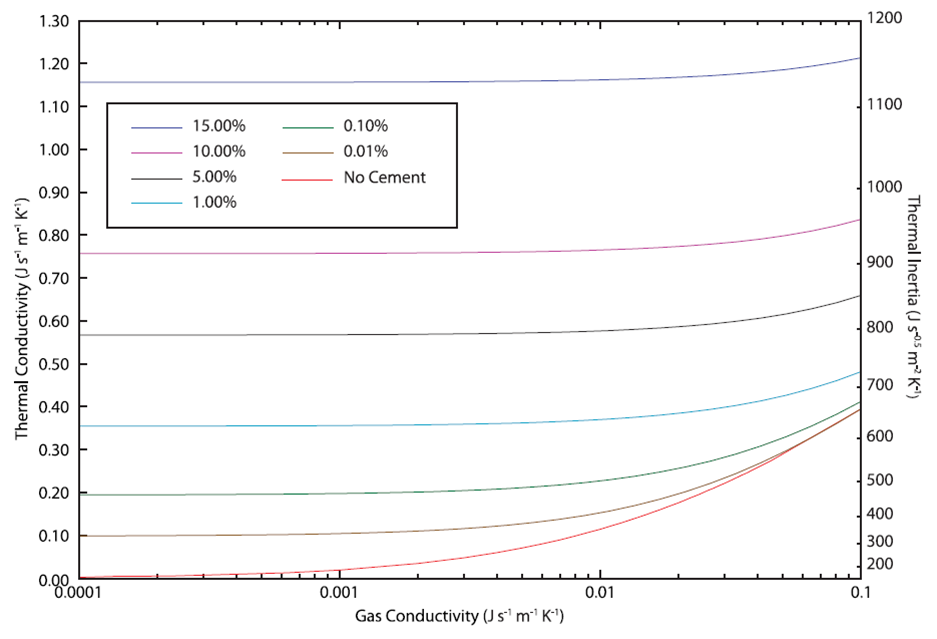
\includegraphics[scale=0.5]{PandQ2009b_CementVolumeFraction.png}

	The image shows that the measured thermal conductivity inside the anomaly ($k_{in} = 0.0113 \: J/(m \cdot s \cdot K)$) falls well below the minimum cement volume fraction used by P and C. However, it can be seen that, for vanishing gas conductivity,  the relationship between the cement volume fraction and thermal conductivity can be approximated by $V_{cem} \varpropto 21\cdot k_{eff}^{3.32}$. Thus, the volume fraction of cement inside and outside the anomaly was estimated as:
	
	\begin{itemize}
	\item $\chi_{in} \approx 7\times10^{-6}\%$
	\item $\chi_{out} \approx 5\times10^{-10}\%$
	\end{itemize}
	
	It should be noted that the grain thermal conductivity used was only 0.937 MKS, while the cement thermal conductivity used in the graph above was 6 MKS. However, the effects of varying these parameters were explored in several other plots in their paper, and it can be seen that for very low cement volume fractions the cement thermal conductivity does not effect the effective thermal conductivity and for all cement thermal conductivities evaluated the effective thermal conductivity approaches a single value dependent on grain size and pore gas pressure. Though the effect of varying the grain thermal conductivity was not discussed in the paper, it can be assumed to be negligible because the effective thermal conductivity is controlled by the cementation between grains. Furthermore, it is stated in the paper that '\emph{for extremely small volumes of bonds ($< 0.01\%-0.001\%$) the bulk thermal conductivity remains mostly unchanged and is a function of ... temperature and grain size}'. We see that the determined values for cement volume fraction are well below these limits, and thus the model of P and Q is not adequate to estimate the cementation between grains. 
	
\subsection{Steiner and K\"{o}mle (1991): Determination of grain sinter radius by Hertz factor analysis}

	A third method of determining the effective thermal conductivity of a porous water ice regolith at low pressure (high Knudsen numbers) was outlined in Steiner and K\"{o}mle (1991) who used expressions given in Tsostas and Martin (1987) to derive:

	\begin{equation}
	k_{eff} = (1-\sqrt{1-\phi})\phi \cdot k_{void} + \sqrt{1-\phi}[hk_{ice}+(1-\phi)\frac{B+1}{B}\frac{k_{ice}k_{void}}{k_{ice}+k_{void}}]
	\end{equation}
	
	where $\phi$ is the regolith porosity, $k_{void}$ is the thermal condictivity across the void region due to a combination of radiative heat transfer and the latent heat of sublimation, $k_{ice}$ is the thermal conductivity of bulk ice, h is the 'Hertz-factor' used to describe the amount of intergrain contact, and B is a deformation factor related to porosity by:
	
	\begin{equation}
	B = 1.25 ( \frac{1-\phi}{\phi} )^{10/9}
	\end{equation}
	
	The Hertz-factor is a parameter that describes the intergranular contact area, where a larger Hertz-factor corresponds to greater interparticle contact, thereby allowing a greater heat flux and a higher thermal conductivity. That is, for otherwise identical regoliths, the Hertz factor is a parameter that can be used to describe the relative(?) amount of granular cementation. Using the greater value of $k_{void} = 6.3\times10^{-6} \frac{J}{m \cdot s \cdot K}$ from the analysis above and a thermal conductivity for ice at 80 K of $k_{ice} = 567/T = 7.09 \frac{J}{m \cdot s \cdot K}$, we can analyze the effective thermal conductivity to obtain a comparison of the Hertz factor inside and outside the thermal anomally feature.
	
	Noting that for a porosity of $\phi = 0.5$, the deformation factor $B = 1.25$, and thus the effective thermal conductivity can be reduced to:
	
	\begin{equation}
	\begin{split}
	k_{eff} = (1-\sqrt{1-0.5})(0.5)(6.3\times10^{-6}) + &\sqrt{1-0.5} [ H \cdot 7.09+(1-0.5)\frac{1.25+1}{1.25}\frac{(7.09)(6.3\times10^{-6})}{(7.09+6.3\times10^{-6})} ] \\
	\Rightarrow k_{eff} &= ( 4.93\times 10^{-6} + 2.24\cdot H )  \frac{J}{m \cdot s \cdot K} \\
	\text{or} \: k_{eff} &\approx \sqrt{1-\phi}\cdot H \cdot k_{ice}(T)
	\end{split}
	\end{equation}
	
	That is, we can effectively ignore the contributions due to radiative or latent hear effects, and consider only the thermal conductivity due to conduction through the grains. Taking the effective thermal conductivities obtained above for the regolith inside and outside the anomaly, we can solve for the Hertz-factor:
	
	\begin{itemize}
	\item $k_{in} = 1.13\times10^{-2} \frac{J}{m \cdot s \cdot K} \Rightarrow H_{in} = 0.00225$
	\item $k_{in} = 6.64\times10^{-4} \frac{J}{m \cdot s \cdot K} \Rightarrow H_{out} = 0.00013$
	\end{itemize}
	
	Here it is worthwhile to note that Hertz-factors used previously in the literature to describe a porous icy cometary nucleus are on the order of  $H  \approx (1 - 4) \times10^{-3}$ [SteinerKomle1991], which compares favorably with the values obtained for the Mimas regolith. 
	
\subsubsection{What is the Hertz-factor really?}

	In modeling of thermal conductivity of grainy, porous materials, a common approximate technique is to consider a mono- or polydisperse 'bed' of elastic spheres. The requirement for the spheres to be elastic and not a perfect hard sphere stems from physical considerations, since the contact point of hard spheres is infinitesimal, through which no heat can flow. Therefore, the spheres must deform slightly at the contact point so there is some finite area across which heat can flow. At the atomic scale, the heat transfer through disimilar spheres with no adhesive bonding is due predominantly to the van der Waals intereactions which mediate the phonon transfer, while for cemented grains where there is adhesive material connecting the grains which tranfer heat directly through lattice vibrations. 
	Experimentally, the thermal conductivity is seen to depend exponentially on the volume filling factor $\vf = 1- \phi$, determined experimentally by taking the mass of a given volume of grainy material and comparing to the volume of an equivalent mass of solid material, as [Krause et al, 2011 (via Gundlach and Blum (2012))],:
	
	\begin{equation}
	k(\vf) = c_{1} exp [c_{2} \vf]
	\end{equation}

	where $c_{1}$ and $c_{2}$ are derived by fitting the measured data.
	
	Theoretically, the thermal conductivity of elastic spheres can be explained using the Hertzian theory of contact [Hertz, 1881] to describe the deformation of the interface between spheres. For packed spheres under vacuum ($k_{cond} = 0$), the heat conductivity can be calculated by [ChanTien1973]:
	
	\begin{equation}
	k_{eff}(r, T, \vf) = k_{ice}\cdot \sr_{contact}\cdot \xi(r, \vf)= k_{ice}(T) [\frac{3}{4} \frac{1 - \mu^{2}}{E(T)} F(r) r]^{1/3} \xi(r, \vf)
	\end{equation}
	
	 where $r$ is the particle radius, $k_{ice}$ is the thermal conductivity of bulk (solid) ice, $\sr$ is the radius of the contact area between touching spheres as described by the Hertz relation, $\mu$ and $E(T)$ are Poisson's ratio and Young's modulus of the material, respectively, and $F(r)$ is an externally applied force which acts on the spheres and determines the contact area between adjacent particles. The packing structure of the material and the number of interparticle contacts is taken into account by $\xi(r, \vf)$ where:
	
	\begin{equation}
	\xi(r, \vf) = \frac{1}{0.531 S(\vf)} \frac{N_{A}(r)}{N_{L}(r)}
	\end{equation}
	 
	 Here, $s(\vf)$ is a 'model parameter' that depends on the packing structure, and $N_{A}(r)$ and $N_{L}(r)$ are the number of particles per unit area and unit length respectivenly.  When no external force is applied, the weight of the particles can be used to determines the force and thus the contact area, but van der Waals bonding can provide orders of magnitude greater adhesive forces and it can be calculated by the JKR theory [Johnson et al (1971)] as:
	 
	 \begin{equation}
	 F_{vdW}(r, T) = 3 \pi \gamma(T) r
	 \end{equation} 
	 
	 where $\gamma(T)$ is the specific surface energy of the material and a measure of the adhesive bonding strength between grain surfaces. It should be noted here that this expression may differ substantially for sintered grains where the boundary may have some degree of crystalline bonding. Substituting the above expression into the conductivity equation, we can define the Hertz-factor as the ratio of the effective (regolith) thermal conductivity and the bulk conductivity:
	 
	 \begin{equation}
	 \label{eq:hertz}
	 H(r, T, \vf) = \frac{k_{eff}(r, T, \vf)}{k_{ice}(T)} = [\frac{9}{4} \frac{1-\mu^{2}}{E(T)} \pi \gamma(T) r^{2} ]^{1/3} \xi(r, \vf)
	 \end{equation}
	 
	 This equation can be modified to describe a porous regolith layer composed not simply of spherical grains, but of grain aggregates which themsleves are composed of ice grains and which have their own unique materials parameters such as volume filling factor, Poisson's ratio, Young's modulus, and specific surface energy. Taking the volume filling factor of the layer to be the product of the volume filling factors of the aggregates themselves (\vf$_{agg}$) and the volume filling factor of the aggregate structure \vf$_{struc}$), i.e. ($V_{F, layer} = V_{F, agg} V_{F, struc}$, we can write the effective thermal conductivity of the layer as:
	 
	 \begin{equation}
	 \begin{split}
	 k_{layer}(r_{0}, R, T, V_{F, struc}, V_{F, agg}) = \\
	 k_{agg}(r_{0}, T, V_{F, agg}) [\frac{9}{4} \frac{1 - \mu_{agg}^{2}}{E_{agg}(T)}  \pi \gamma_{agg}(T) r^{2}]^{1/3} \xi(R, V_{F, struc})
	 \end{split}
	 \end{equation}
	 
	 where $R$, $E_{agg}$, and $\mu_{agg}$ are the radius, Young's modulus, and Poisson's ratio of the aggregates, respectively. Taking $r_{0}$ to be the grain radius (the size of the grains that make up the aggregate), the specific surface energy of the aggregates can be calculated by:
	 
	 \begin{equation}
	 \gamma_{agg}(T) = V_{F, agg} \gamma_{ice}^{5/3}(T)[\frac{9 \pi (1-\mu_{agg}^{2})}{r_{0} E_{ice}(T)}]^(2/3)
	 \end{equation}
	 
	 The thermal conductivity of the aggregates can be calculated as before:
	 
	 \begin{equation}
	 k_{eff}(r_{0}, T, V_{F, agg} = k_{ice}(T) [\frac{9 (1-\mu_{ice}^{2})}{4 E_{ice}(T)}\pi \gamma_{ice}(T) r_{0}^{2} ]^{1/3}\xi(r_{0}, V_{F, agg})
	 \end{equation}
	 
	\emph{ In this expression, the unknown parameters are the volume filling factors, assuming that materials parameters can be found for both the bulk material and the aggregates.}
	
\subsection{Sirono and Yamamoto (1997):}

	Using effective-medium theory, the effective thermal conductivity for a random network of spherical grains arranged on a regular lattice can be determined by integrating the propability distribution of $k$ multiplied by the 1-D heat flux to obtain the effective heat flux, which then yields(Eq. 8 of Sirono and Yamamoto):
	
	 \begin{equation}
	 \frac{k_{eff} - k_{ice}}{k_{ice} +(1/p_{c}-1)k_{eff}}p + \frac{k_{eff}-k_{void}}{k_{void}+(1/p_{c}-1)k_{eff}}(1-p)=0
	 \end{equation}

	 where the probability of a lattice site being occupied or packing fraction is $p$, $p_{c}$  is the percolation thereshold which defines the minimum packing fraction for a continuous thermal path to exist across the material, and $k_{eff}$, $k_{ice}$, and $k_{void}$ are the effective, bulk ice, and void space thermal conductivities respectively. If we take $k_{void} \approx 0$, this equation reduces to:
	 
	 \begin{equation}
	 k_{eff} = k_{ice} \frac{p - p_{c}}{1 - p_{c}}
	 \end{equation}
	 
	 However, this expression does not account for the constuction of heat flow due to reduced area at the grain contacts, and this effect can be taken into account by multiplying by a factor that takes into account the contact area, packing structure, and grain size. The contact area in turn is determined Hertzian analysis
	 
		\begin{equation}
		\begin{split}
		k_{eff} &= k_{ice} ( \frac{p - p_{c}}{1-p_{c}} )\frac{\pi \sr^{2}}{g r^{2}} \\
			 &= k_{ice} ( \frac{p - p_{c}}{1-p_{c}} )\frac{\pi}{g r^{2}}[ \frac{9 \pi \gamma r^{2} (1-\mu^{2})}{8 E} ]^{2/3}
		\end{split}
		\end{equation}
	
	
\section{Estimaters based on the models above}
	
\subsection{Grain size comparisson via. Hertz-factor analysis}
	
	If we compare the Hertz-factor as defined by the ratio of the effective and bulk thermal conductivities ~\eqref{eq:hertz}, assuming that the materials parameters ($\mu, E, \gamma$) as well as the packing structure are the same inside and outside the anomaly, the ratio of the grain size inside and outside the anomaly can be determined as:
	
	\begin{equation}
	\begin{split}
	\frac{H_{in}}{H_{out}} &= \frac{k_{in}}{k_{out}} = \frac{r_{in}^{2/3} \xi(r_{in}, \vf)}{r_{out}^{2/3} \xi(r_{out}, \vf)} \\
	\Rightarrow \frac{H_{in}}{H_{out}} &= \frac{r_{in}^{2/3} \frac{N_{A}(r_{in})}{N_{L}(r_{in})}}{r_{out}^{2/3} \frac{N_{A}(r_{out})}{N_{L}(r_{out})}} \\
	& \text{where }\: N_{A}\varpropto \frac{1}{r^{2}} \: \text{and} \: N_{L}\varpropto \frac{1}{r} \\
	\Rightarrow \frac{r_{in}}{r_{out}} &= (\frac{H_{out}}{H_{in}})^{3}
	\end{split}
	\end{equation}
	
	Based on the Hertz-factor analysis, it is seen that the thermal conductivity $k_{cond} \varpropto \frac{1}{r^{1/3}}$, while the thermal conductivity due to radiative heat transfer $k_{rad} \varpropto r$. Therefore, at high temperatures the radiative term will dominate and the thermal conductivity will increase. However, at lower temperatures the radiative contribution is negligible and the thermal conductivity will increase with decreasing particle size, possible due to the increased number of interparticle contacts. 
	
	\begin{equation}
	 \frac{r_{in}}{r_{out}} = (\frac{H_{out}}{H_{in}})^{3} = \fbox{0.00013}
	 \end{equation}

	This comparison estimates that the particle size within the anomaly is ~4 orders of magnitude smaller than the particle size within the anomaly, while comparisons of the measured grain size yield at most a factor of eight (8) difference. Therefore, we can conclude that the variation in thermal conductivity is not due to grain size differences. 
	
\subsection{Using the Hertz-factor to compare cementation radius}

\subsubsection{Kossacki et al, 1994}

	The following equation is given in Kossacki et al (1994) without proof, where $\sr_{n}$ is the cementation (pendular ring) neck radius, and $H_{0}$ is the initial Hertz factor. If we take the 'initial' value to represent the regolith outside of the anomalous region, we have:
	
	\begin{equation}
	\begin{split}
	H &= H_{0} (\frac{\sr_{n}}{\sr_{n,0}})^{2} \\
	\Rightarrow \frac{\sr_{n, in}}{\sr_{n, out}} &= (\frac{H_{n, in}}{H_{n, out}})^{1/2} = 4.17
	\end{split}
	\end{equation}
	
	We see that the contact area inside the anomalous region is greater than without, which is in agreement with the increased thermal conductivity for all other factors being constant. 
	
\subsubsection{Sirono and Yamamoto, 1997}

	The analysis of Sirono and Yamamoto discusses the contact area explicitly. Assuming a simple cubic packing structure of the grains, the give the relation between porosity and the packing fraction as 
	
	\begin{equation}
	\begin{split}
	p &= [ \frac{4}{3} \pi ( \frac{1}{2})^{3} ]^{-1} (1 - \phi) \\
	\Rightarrow \text{for } \phi = 0.5 \text{, } p = 0.955
	\end{split}
	\end{equation}
	
	and the critical packing fraction as $p_{c} = 1/3$ and $g = 4$. 
	
	Calculating the contact areas, we find:
	
	\begin{equation}
	\begin{split}
	S_{in} &= \frac{k_{eff, in}}{k_{ice}} \frac{1-p_{c}}{p - p_{c}}\cdot g r_{grain}^{2} \\
	&= \frac{0.00113}{7.09} \frac{1-1/3}{0.955-1/3} \cdot (4)(50 \mu m)^2 \\
	\Rightarrow S_{in} &= 1.71\times 10^{-11} m^{2} \\
	\text{and } \Rightarrow S_{out} = 1.00\times 10^{-12} m^{2}
	\end{split}
	\end{equation}
	
	Of course, since $S = \pi \sr^{2}$, we can calculate the ratio of the contact radius inside and outside the anomaly as:
	
	\begin{equation}
	\frac{\sr_{in}}{\sr_{out}} = ( \frac{S_{in}}{S_{out}} )^{1/2} = 4.14
	\end{equation}
	
	which is in very close argreement with the value obtained above! Yay!
	
	It is left to determine the growth mechanism of contact area in order to determine if electron impact heating can explain the increased cementation at the grain interface.  
	

\end{document}